\begin{landscape}
\section{Diagramas}\label{diagramas}

\subsection{Diagrama de Classes}
\begin{figure}[htb]
	\centering
	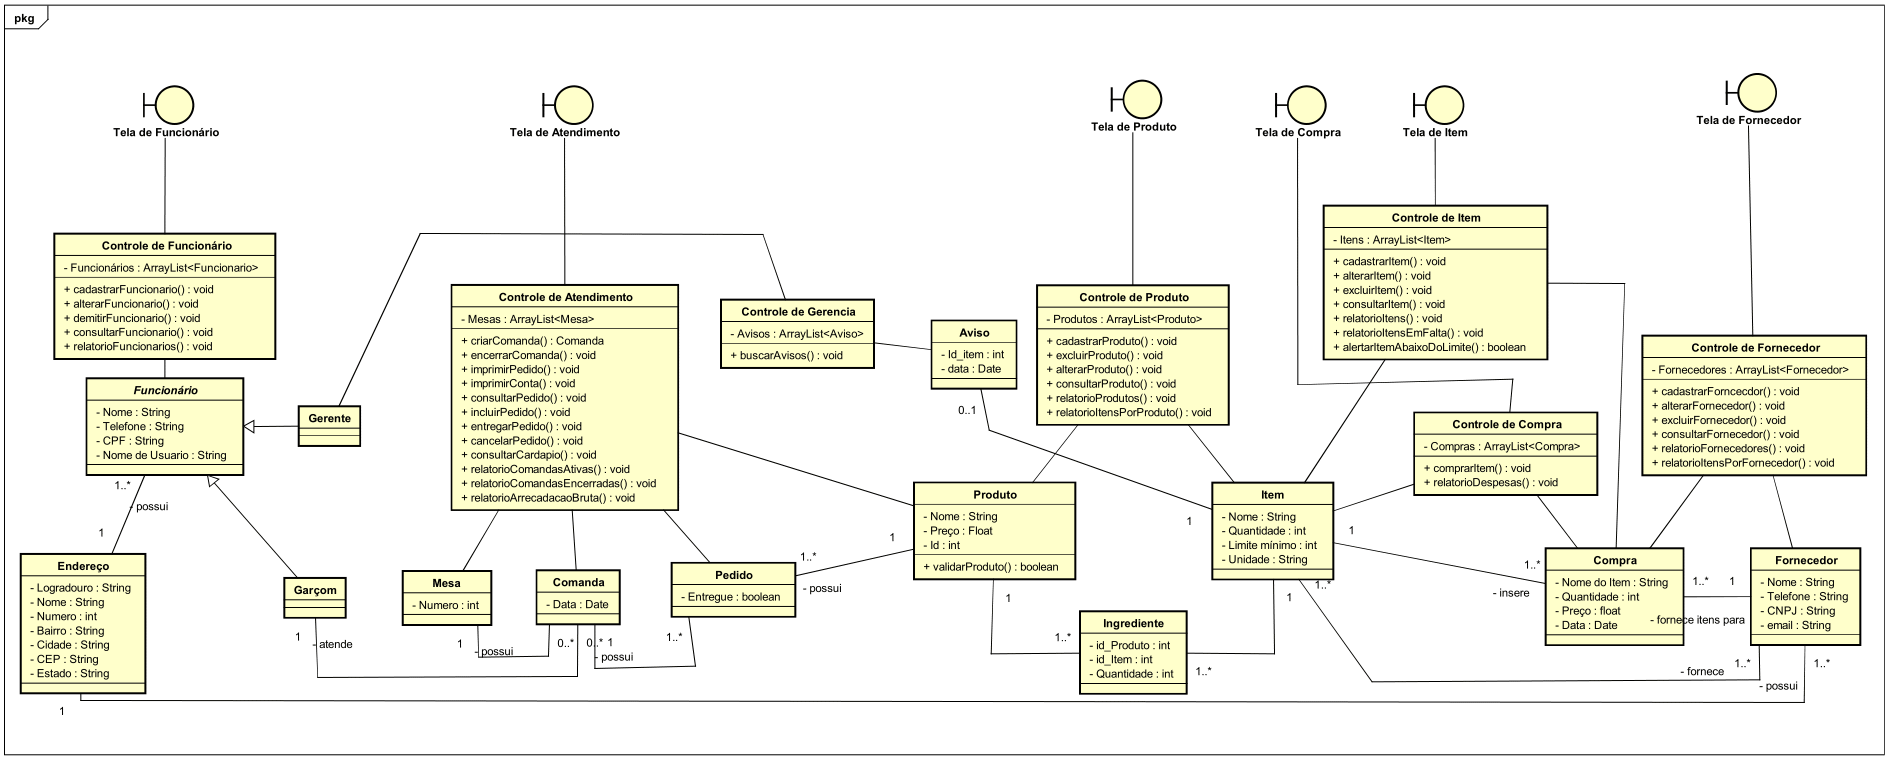
\includegraphics[width=\linewidth,keepaspectratio]{classes.png}
	\caption{Diagrama de Classes}
\end{figure}



\subsection{Diagrama de Sequência}
\begin{figure}[htb]
	\centering
	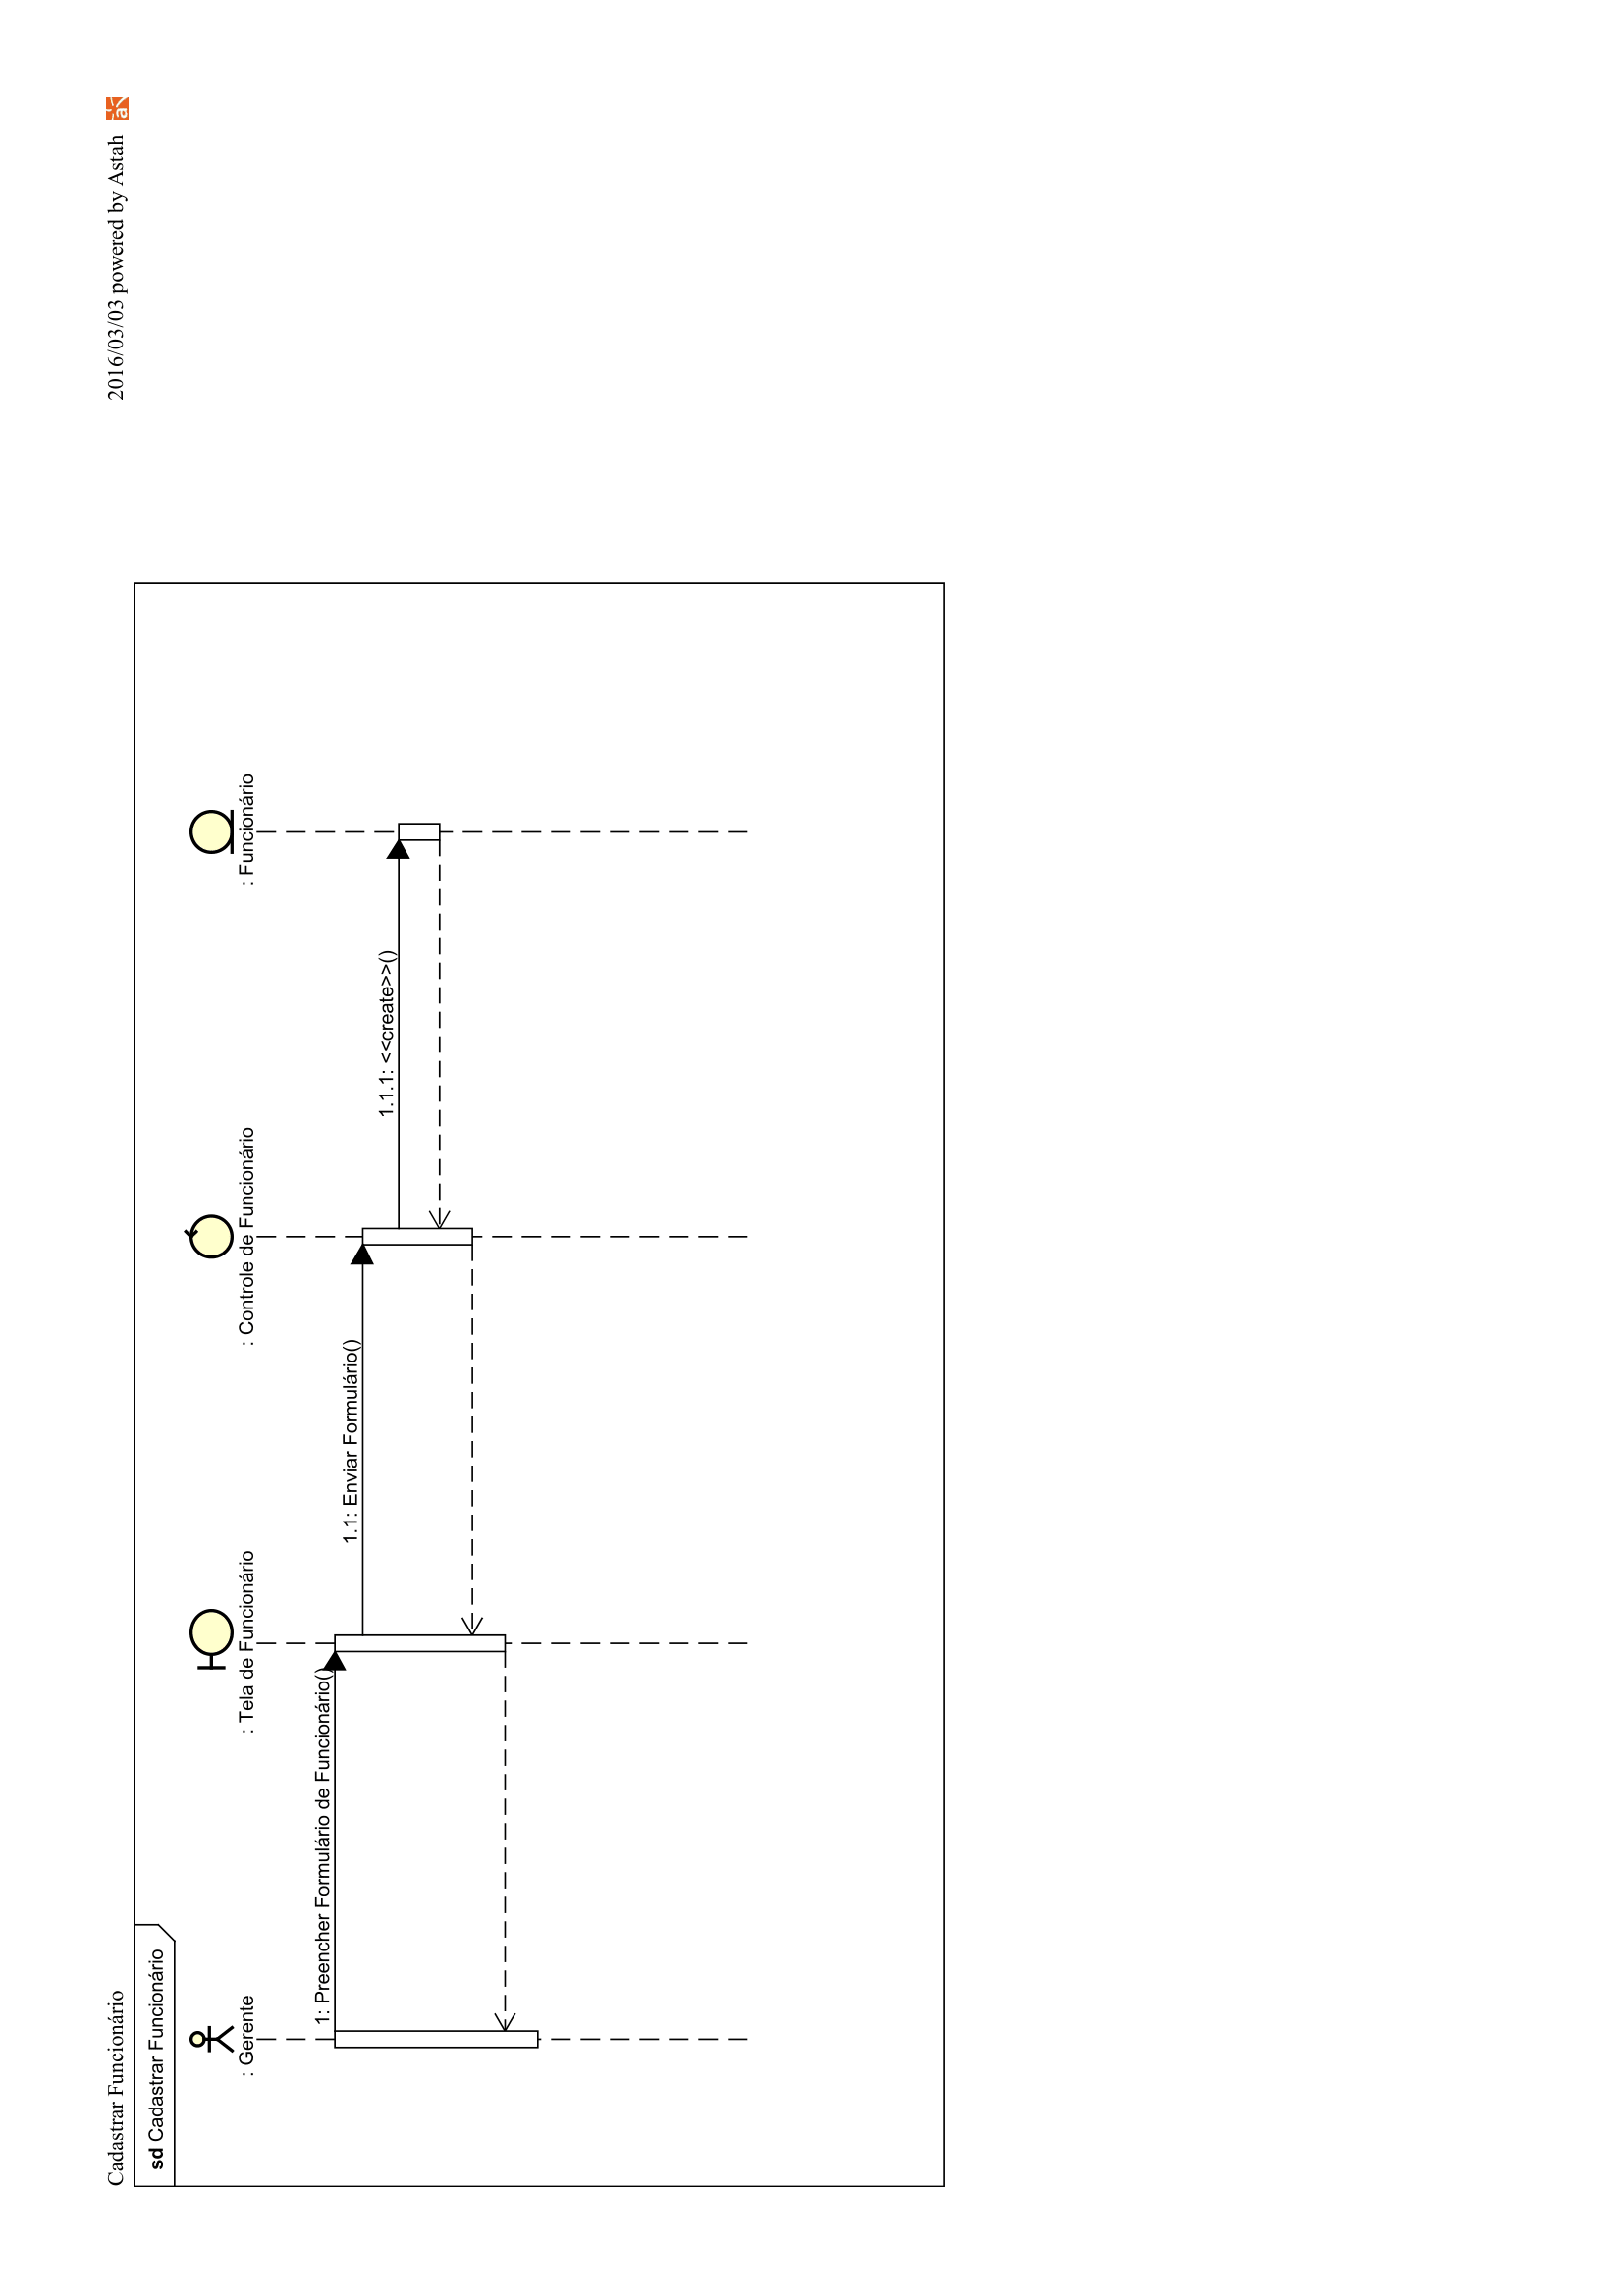
\includegraphics[width=0.85\linewidth,keepaspectratio]{sequencia1.png}
	\caption{Cadastrar Funcionário}
\end{figure}

\begin{figure}[htb]
	\centering
	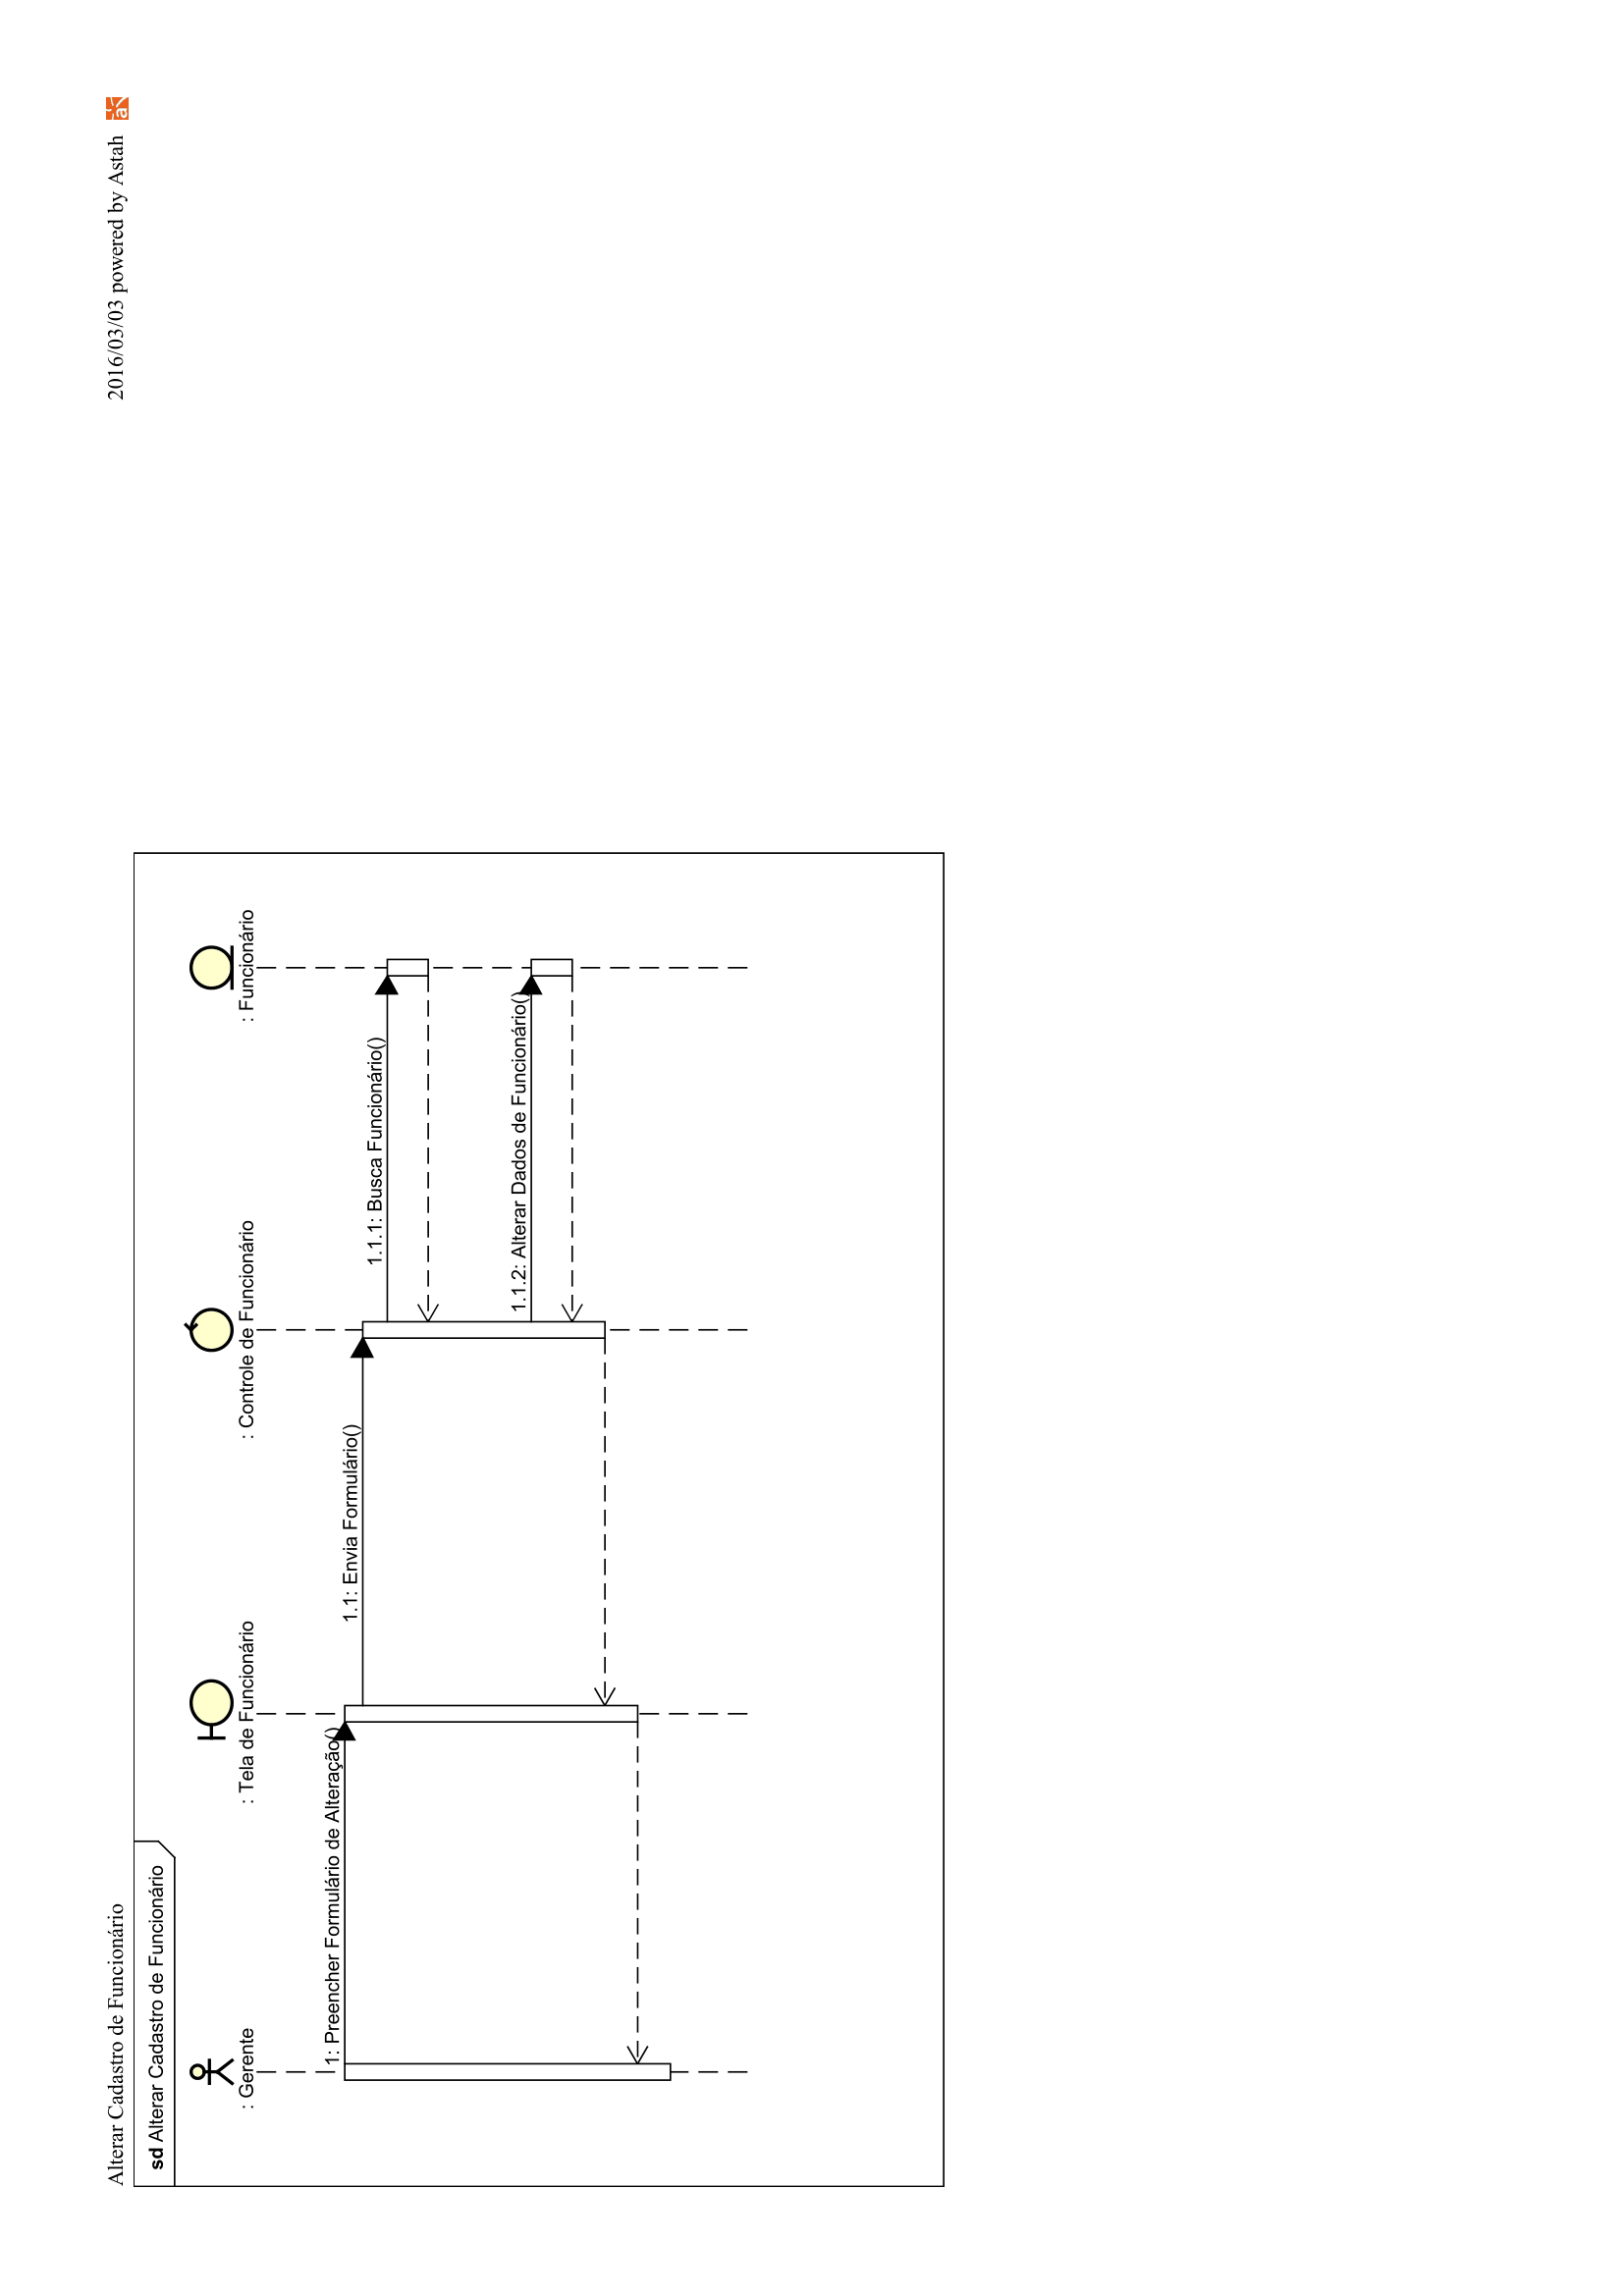
\includegraphics[width=0.85\linewidth,keepaspectratio]{sequencia2.png}
	\caption{Alterar Cadastro de Funcionário}
\end{figure}

\begin{figure}[htb]
	\centering
	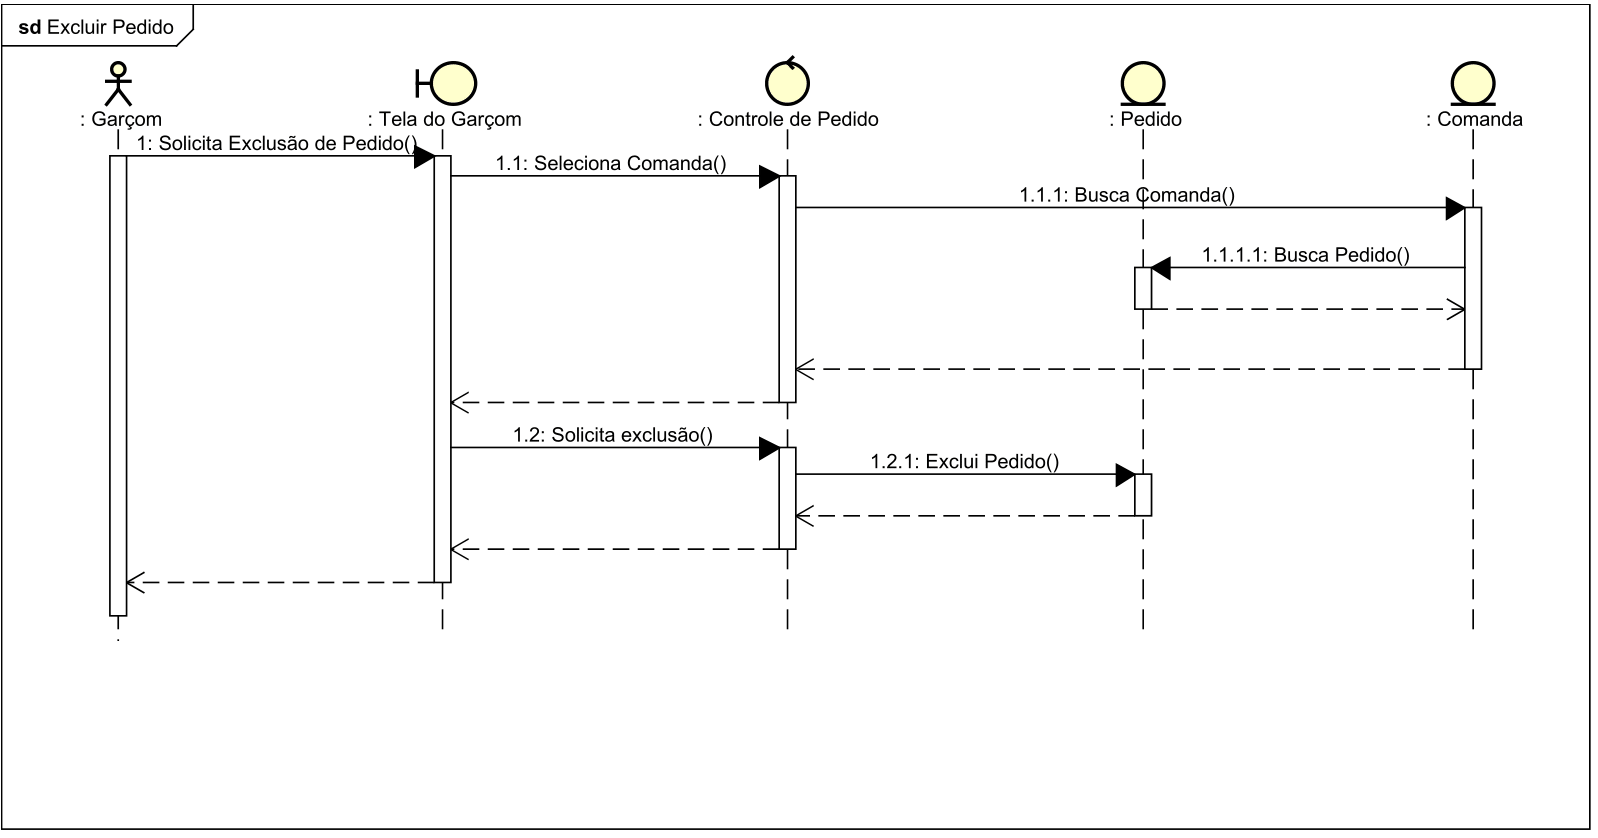
\includegraphics[width=0.85\linewidth,keepaspectratio]{sequencia3.png}
	\caption{Excluir Pedido}
\end{figure}

\begin{figure}[htb]
	\centering
	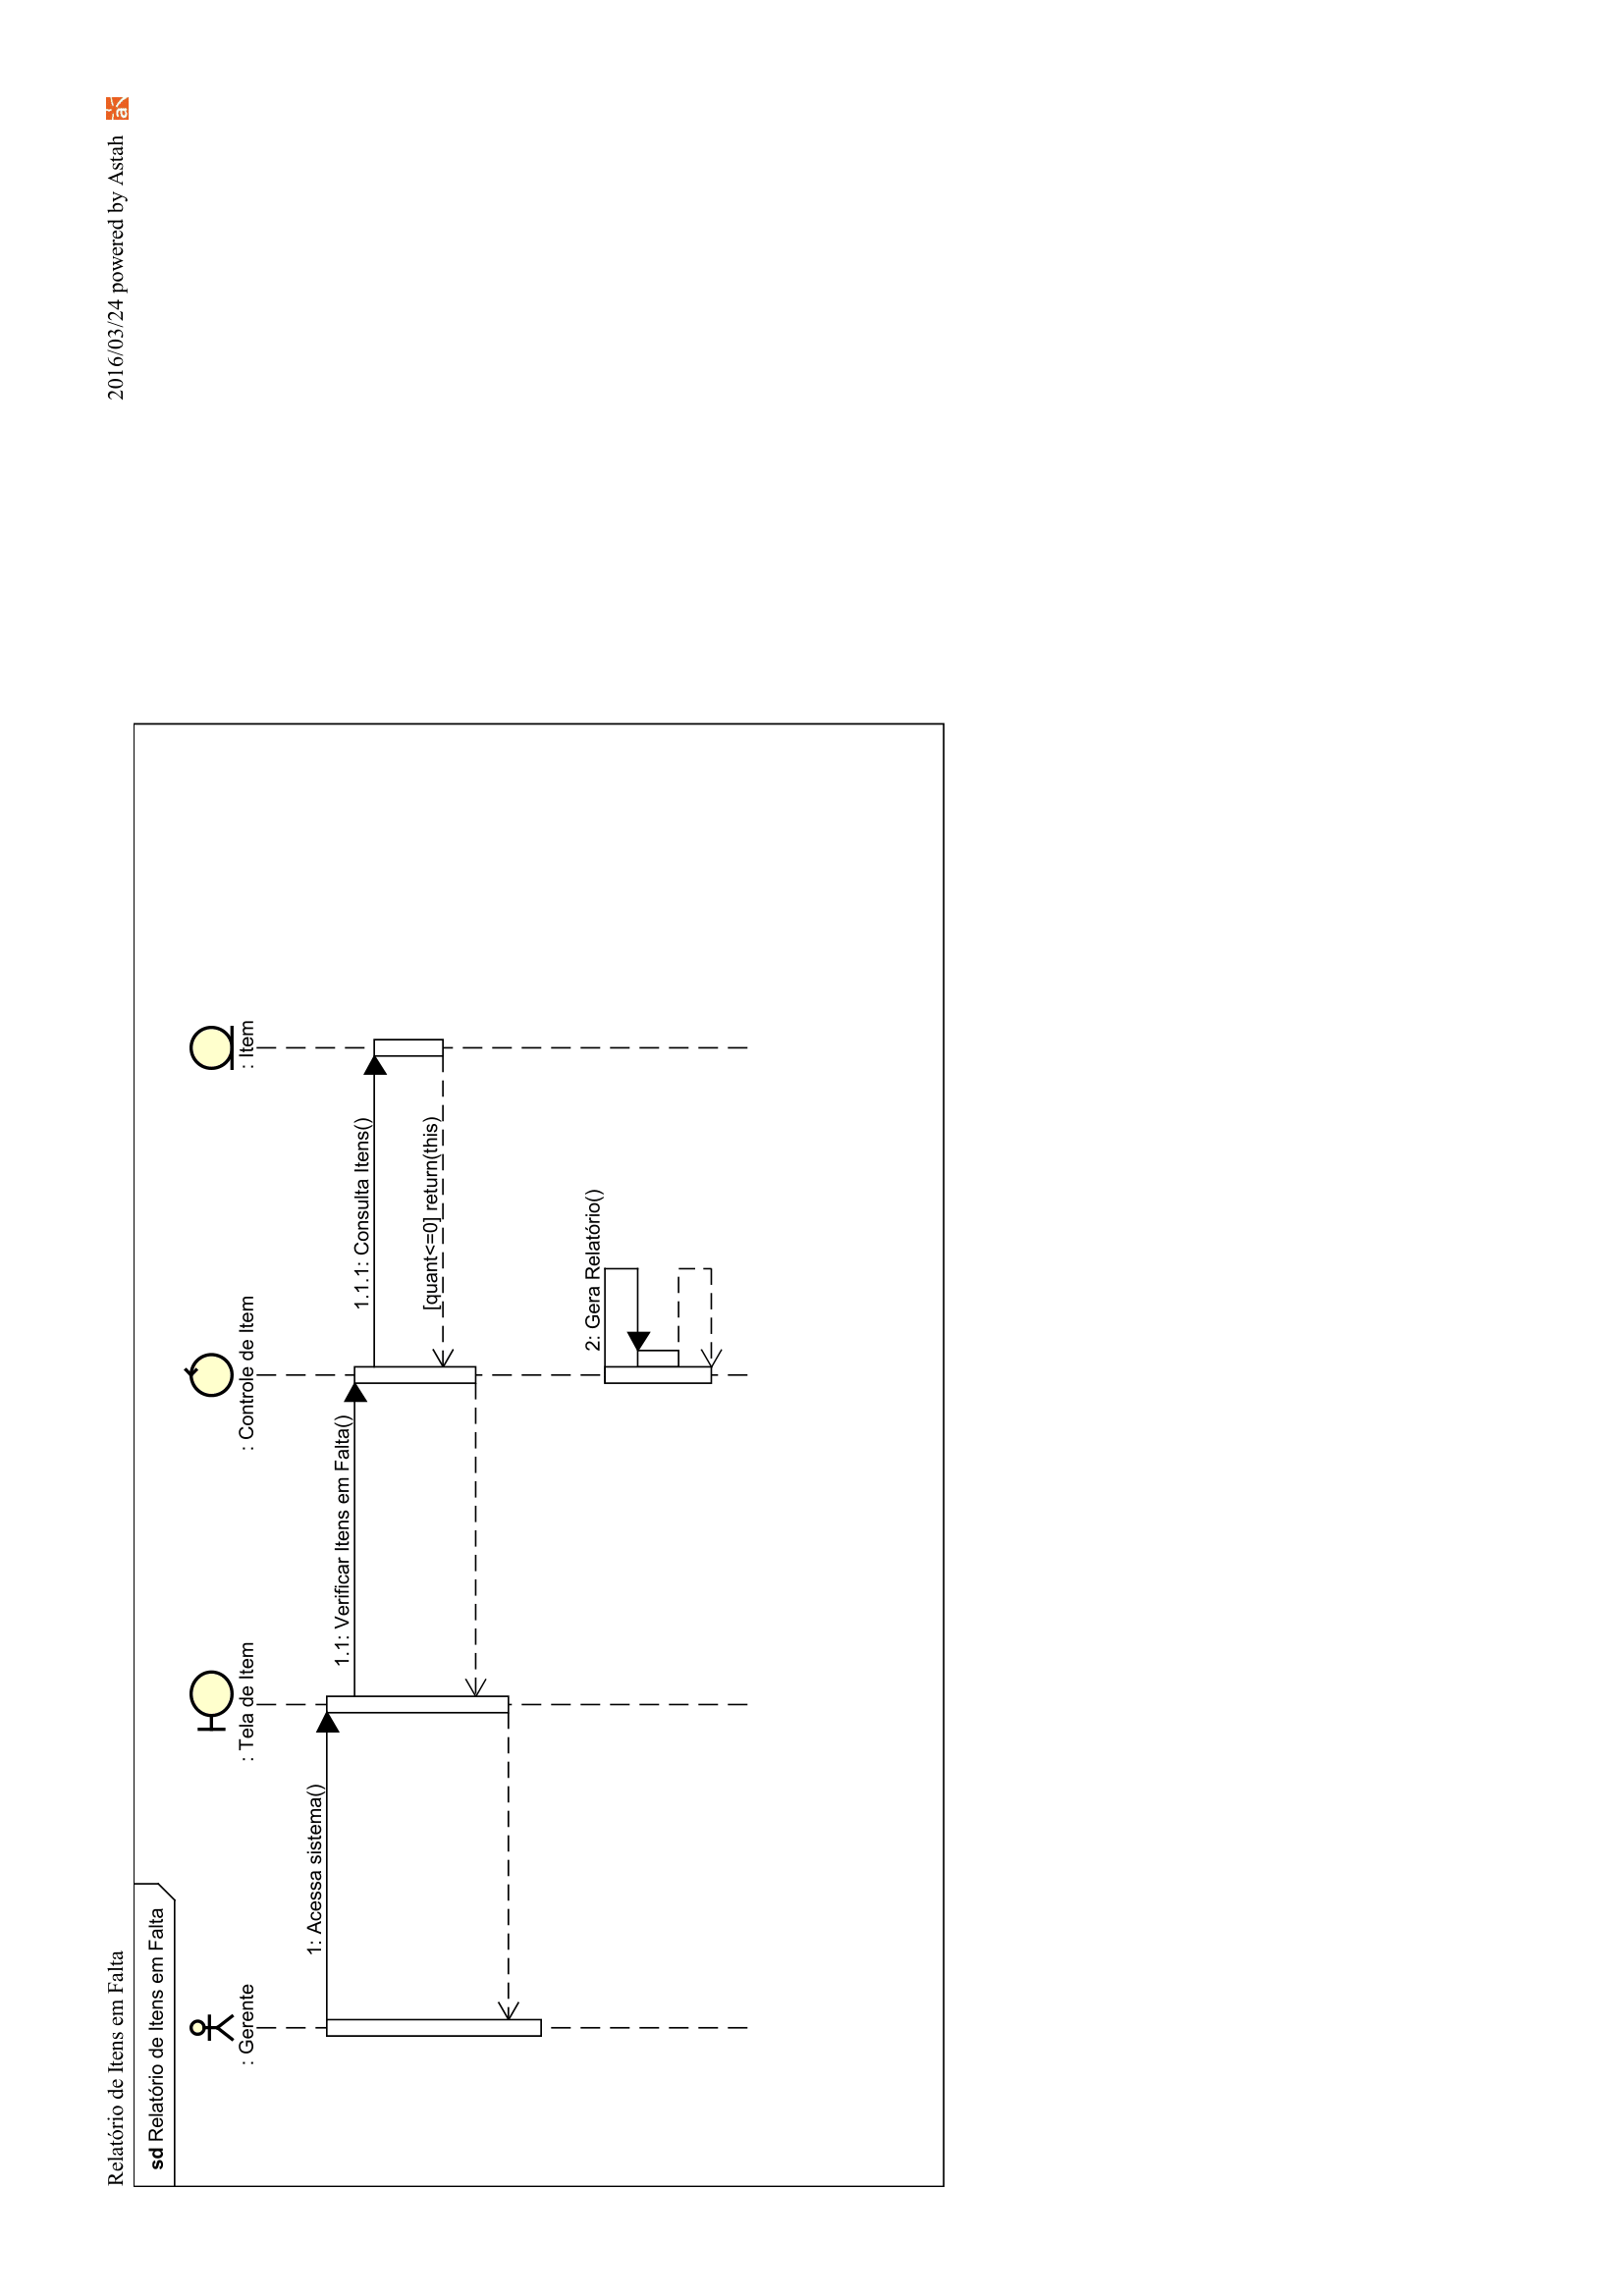
\includegraphics[width=0.85\linewidth,keepaspectratio]{sequencia4.png}
	\caption{Relatório de Itens em Falta}
\end{figure}

\begin{figure}[htb]
	\centering
	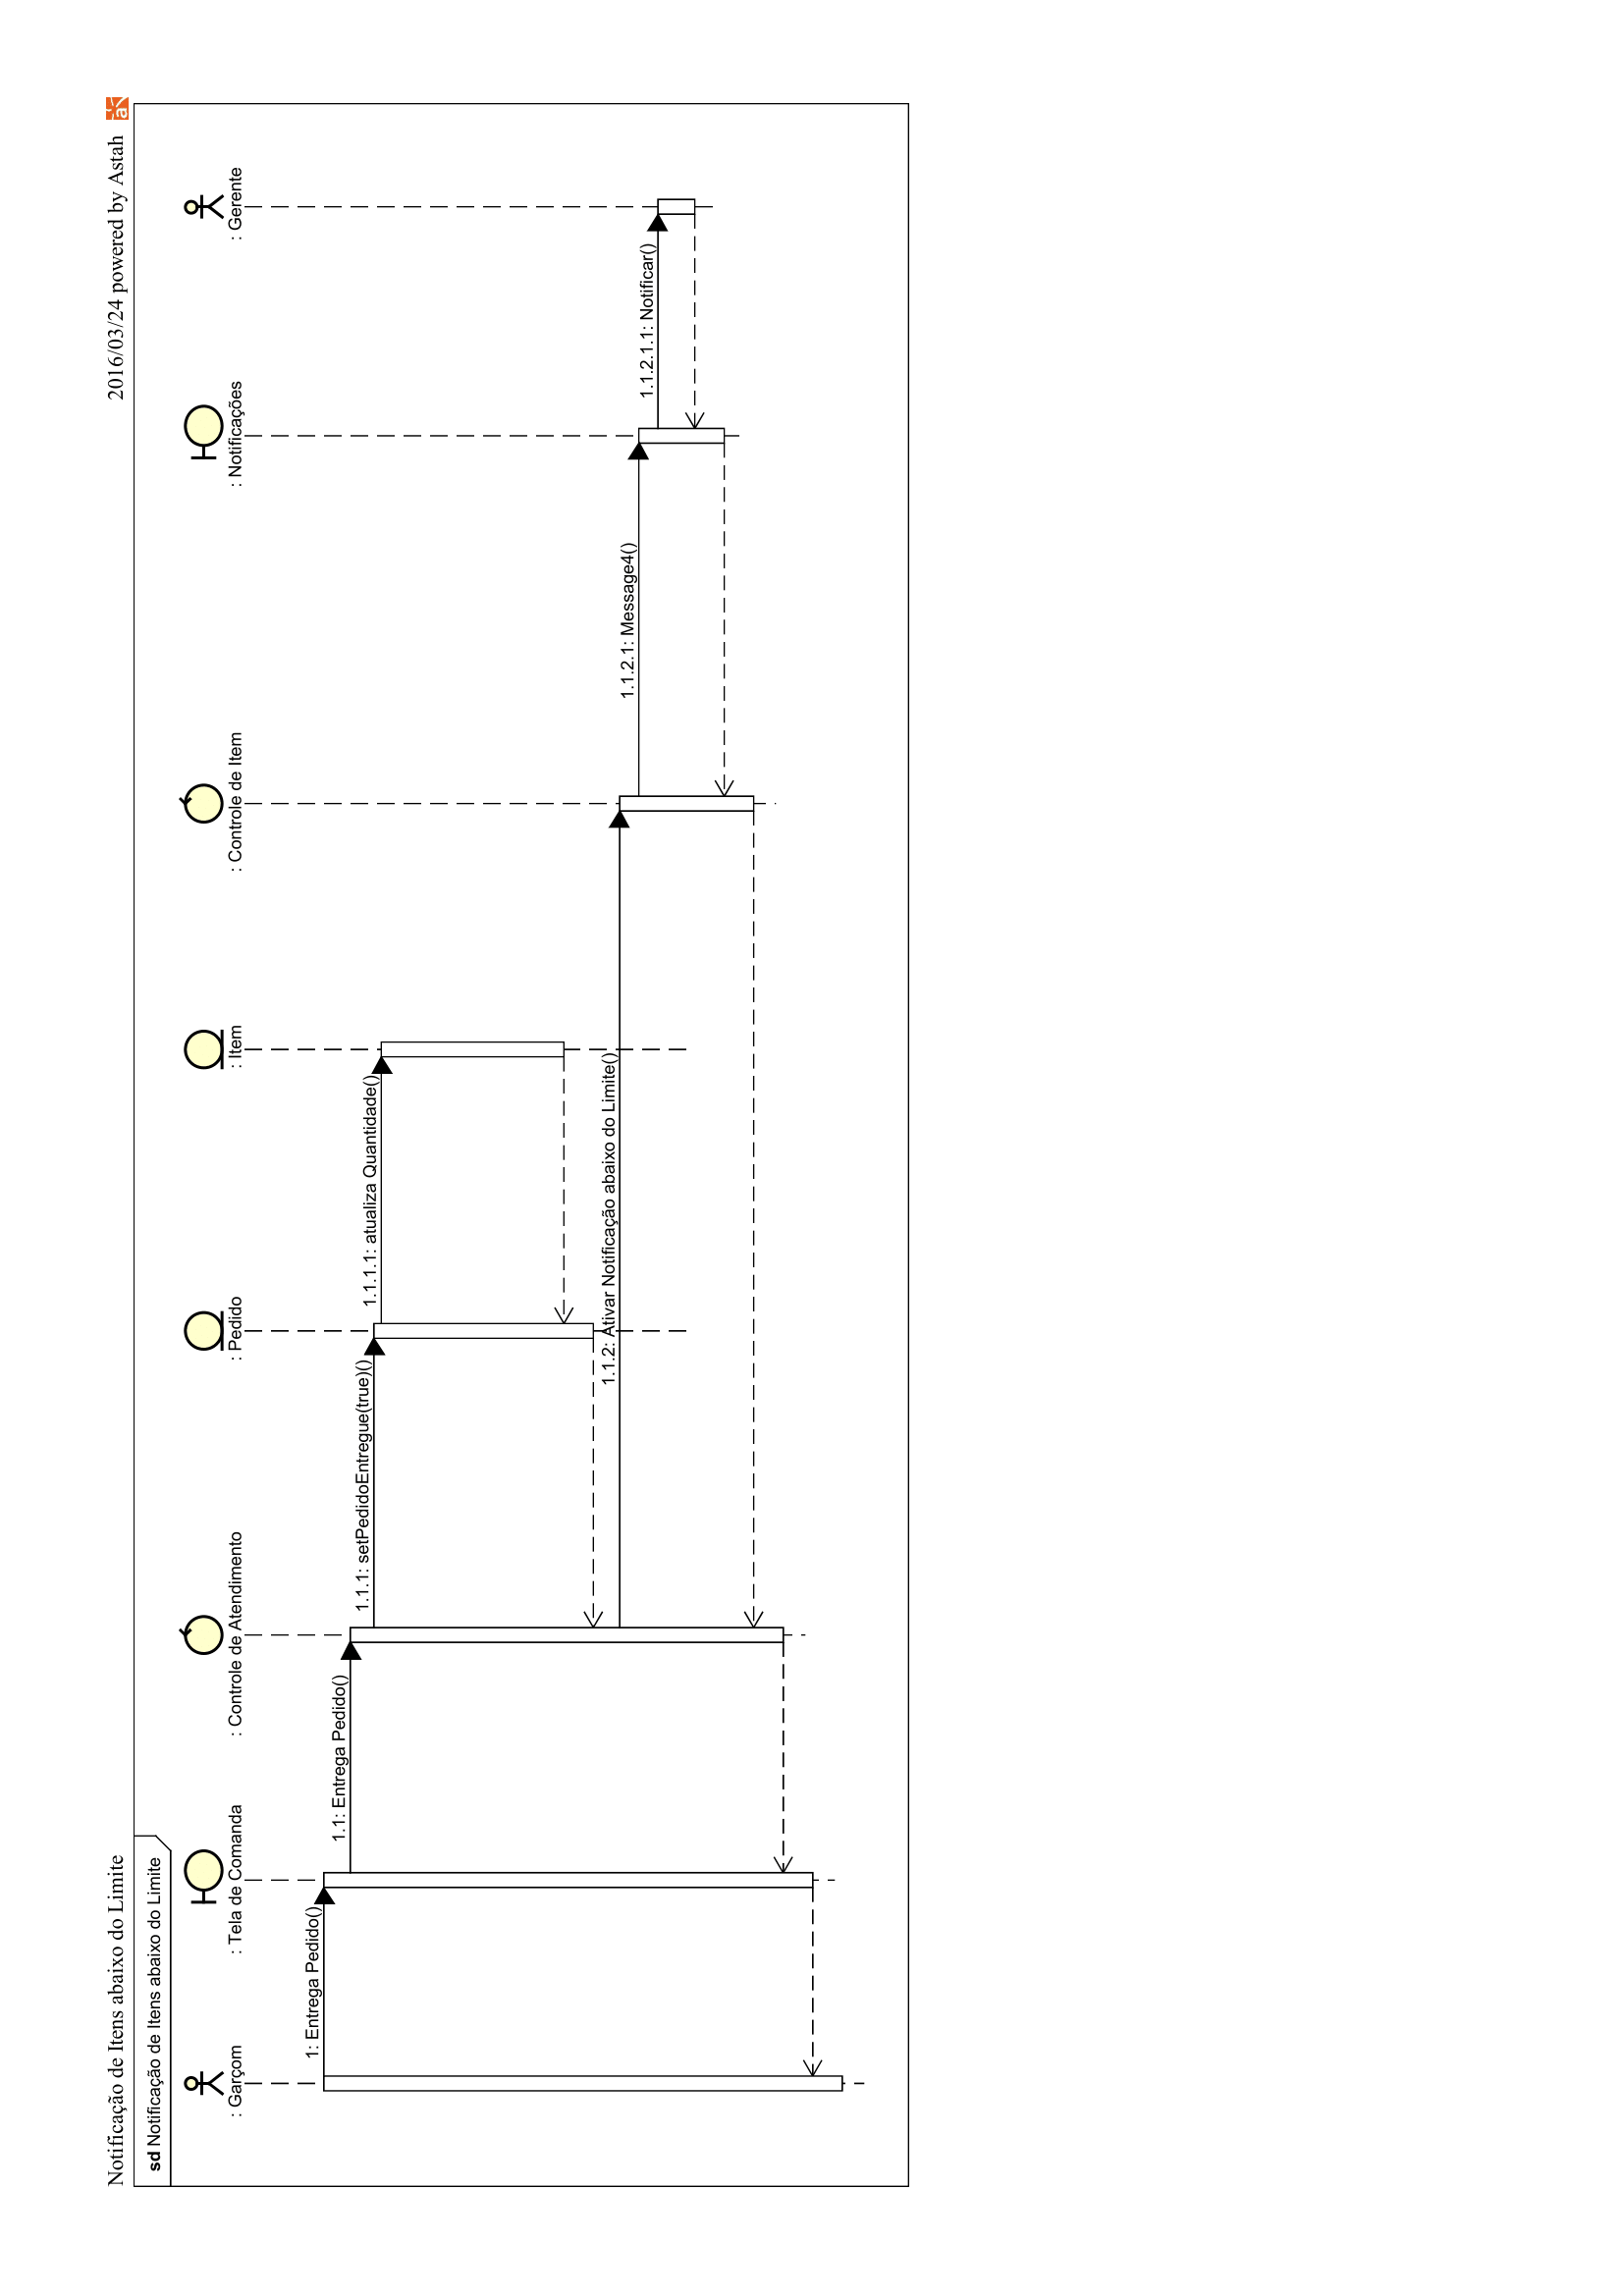
\includegraphics[width=0.85\linewidth,keepaspectratio]{sequencia5.png}
	\caption{Notificação de Itens abaixo do limite}
\end{figure}

\clearpage

\subsection{Diagrama de Casos de Uso}
\begin{figure}[htb]
	\centering
	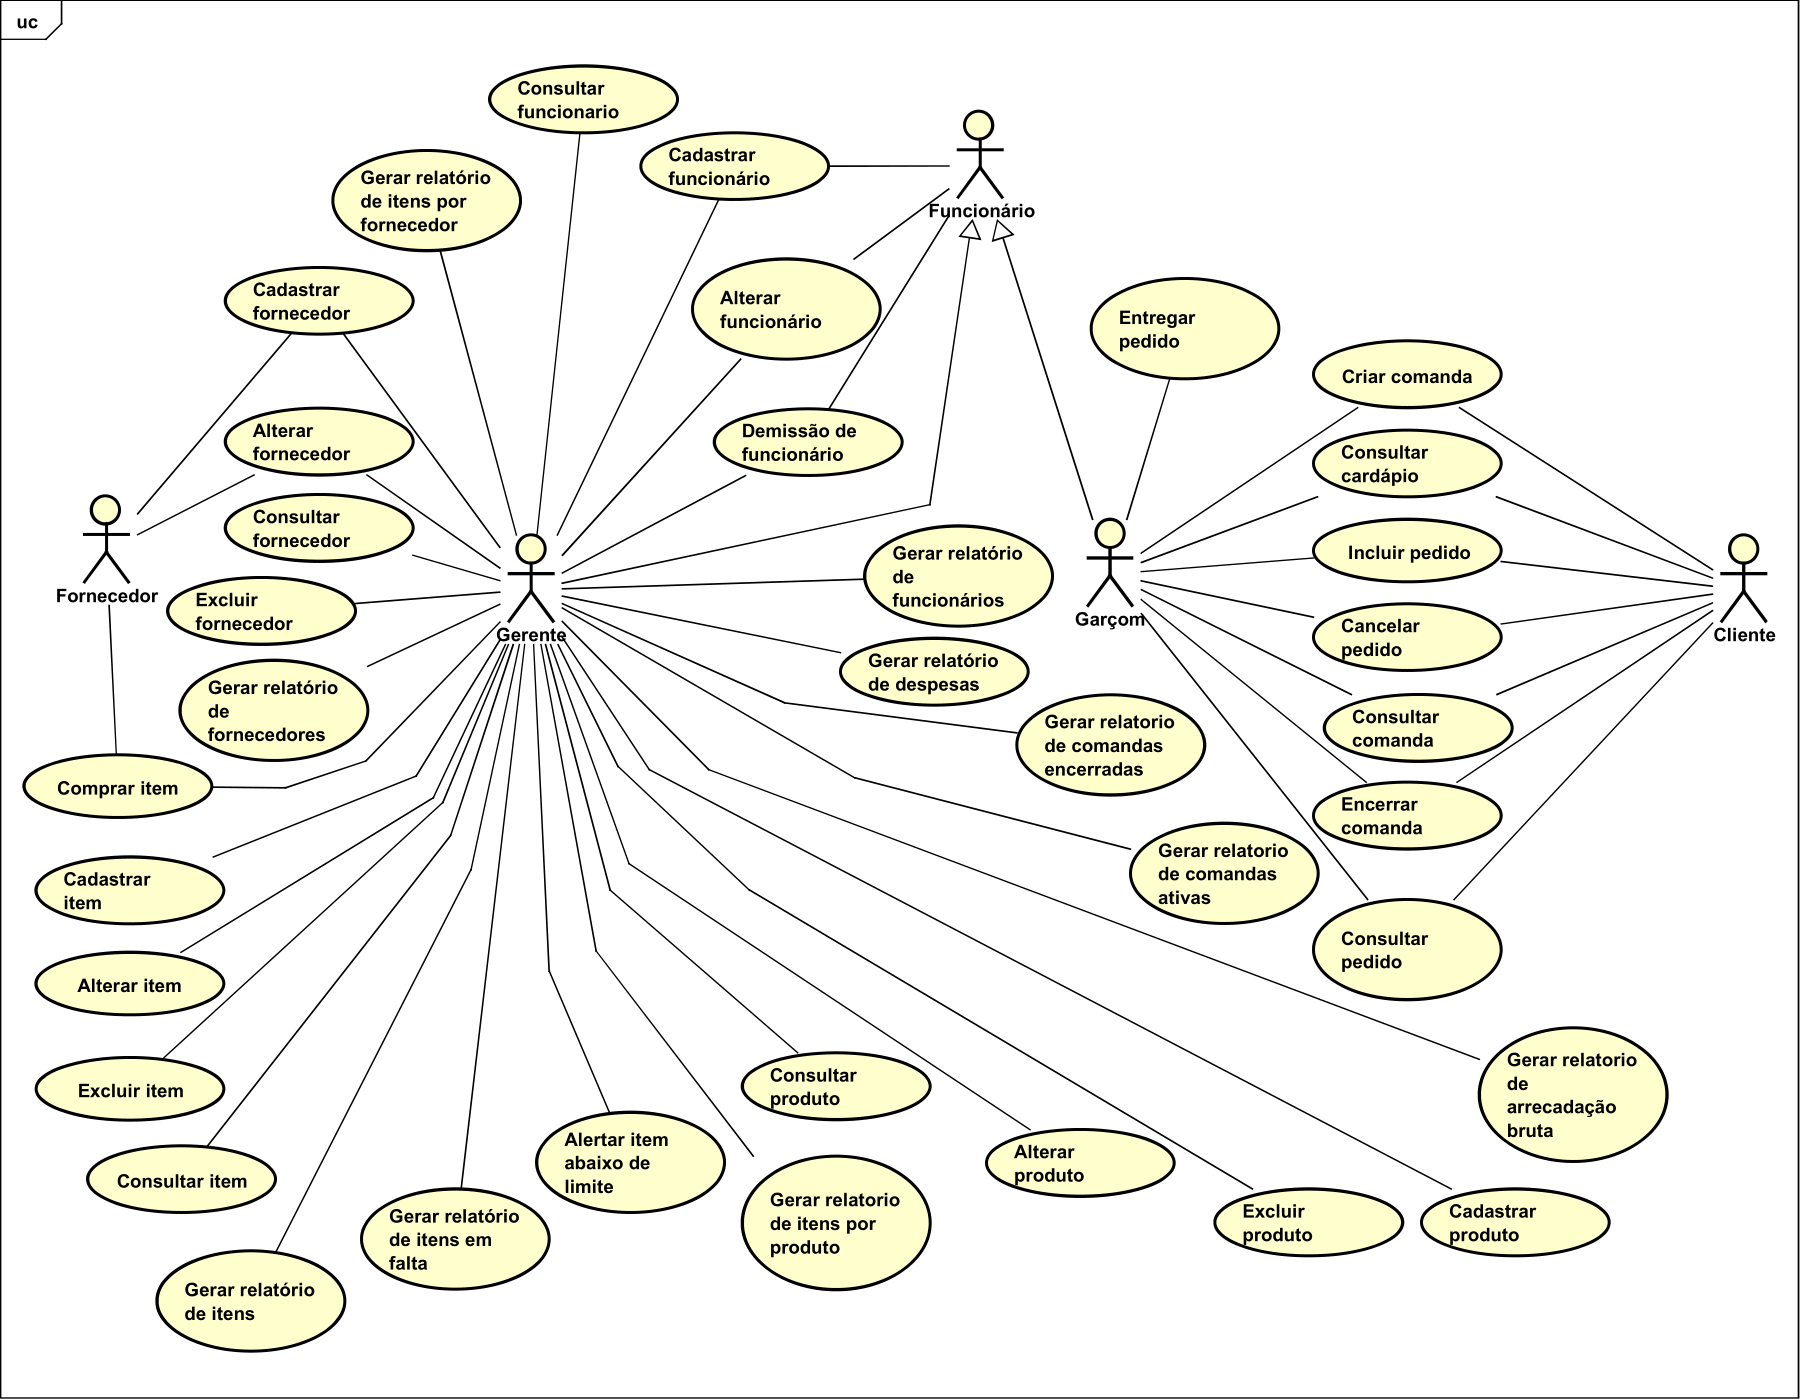
\includegraphics[width=0.75\linewidth,keepaspectratio]{casos_de_uso.png}
	\caption{Diagrama de Casos de Uso}
\end{figure}
\end{landscape}